\documentclass[10pt,letterpaper,oneside]{book}
\usepackage[utf8]{inputenc}
\usepackage[spanish, mexico]{babel} %Para traducir los encabezados al español automáticamente
\usepackage{graphicx} %Para poder incluir un imagen en el documento (tema que se verá a detalle más adelante)
\title{Lugares para visitar en Europa}
\author{Curso de introducción a LaTeX}
\begin{document}
\frontmatter

\maketitle
\tableofcontents

% Capítulos introductorios
\chapter{Introducción}
Europa es un continente grande y rico en historia y cultura, con miles de lugares para visitar, disfrutar, descubrir, aprender, donde descansar o divertirse. Las ciudades europeas tienen siglos de historia, de luchas y enfrentamientos por el poder las cuales han dejado huella en el tiempo y en maravillosas y auténticas obras de arte cultural. Europa tiene impresionantes castillos, imponentes catedrales, palacios señoriales... Por todo lo anterior es muy difícil hacer una lista de 10 ciudades ya que cada ciudad tiene algo especial y con encanto. Por un lado, no es lo mismo que una ciudad sea objetivamente hermosa por su situación, su encanto general y su personal urbanismo o porque tenga hasta media docena de edificios singulares de especial galanura y ello le otorgue mucha categoría. Por otro, los ciudadanos siempre opinarán que la suya es la ciudad más bella, la más limpia, la más divertida, donde mejor se come y se ríe, la más simpática. Entonces, existe un millar de razones, más o menos, para colocar a cualquiera de ellas en un listado de preferencia estética o afectuosa.

% Capítulos del contenido
\mainmatter
    \chapter{Ciudades europeas para vacacionar}
        \section{Viena}
            Viena es una ciudad de Europa Central situada a orillas 
            del Danubio, en el valle de los Bosques de Viena, al 
            pie de las primeras estribaciones de los Alpes. Capital 
            de Austria, así como uno de sus nueve Estados federados
            (Bundesland Wien).\\
 
            Está rodeada por el Estado federado de Baja Austria. 
            Con una población de 1.712.903 habitantes (2010),
            Viena es la mayor ciudad, centro cultural y político 
            de Austria. El área metropolitana cuenta con 2,4 
            millones de habitantes, población similar a la de la 
            ciudad en 1914. El idioma oficial es el alemán.\\
 
        \section{Sevilla}
            Sevilla es un municipio y ciudad española, capital de la 
            provincia homónima y de la comunidad autónoma de Andalucía. 
            Ostenta los títulos de "Muy Noble, Muy Leal, Muy Heroica, 
            Invicta y Mariana Ciudad de Sevilla". Sevilla contaba en 
            2010 con 704.198 habitantes (INE, 2010), siendo la cuarta 
            ciudad de España por población después de Madrid, Barcelona 
            y Valencia.
 
            \subsection*{Catedral}
                La Catedral de Sevilla es la catedral gótica más 
                extensa del mundo y uno de los mayores templos 
                cristianos en cuanto a tamaño, del mundo. Fue declarada 
                por la UNESCO Patrimonio de la Humanidad en 1987.
 
            \subsection*{Giralda}
                La Giralda es el campanario de la Catedral de Sevilla 
                y la torre más representativa de la ciudad. Mide 104 
                metros de altura y fue iniciada en el siglo XII como 
                alminar almohade de la mezquita mayor hoy desaparecida, 
                a imagen y semejanza del alminar de la mezquita Kutubia 
                de Marrakech (Marruecos), no obstante su coronación 
                renacentista y campanario, obra de Hernán Ruiz, fue 
                construida entre 1558 y 1568 por encargo del cabildo 
                catedralicio.
		\section{París}
			París es la capital de Francia, fundada entre los años 250 y 200 a.c. Es una de las mejores y más ricas ciudades del mundo para vivir y visitar. Junto con Londres es considerada el centro económico de Europa. París ha sido considerada durante los últimos siglos como capital del arte y la cultura, conocida popularmente como la Ciudad de la Luz. Numerosos artistas de todas partes del mundo han sentido gran afecto y fascinación por esta ciudad (Monet, Voltaire, Renoir, Sartre, Da Vinci, Van Gogh, Cortázar, Picasso o Wilde). Son muchos sus atractivos turísticos entre los que destacan: La Torre Eiffel, La Catedral de Notre Dame, Los Campos Elíseos, El Campo de Marte, La Santa Capilla, El Palacio Real, La Ópera, Les Halles, El Arco de Triunfo, El Sagrado Corazón, Los Inválidos, El Panteón o el Barrio de Montmartre. Entre sus museos destacan el Museo del Louvre (el museo más famoso y visitado del mundo),el centro de arte moderno Pompidou y el Museo de Orsay. El río Sena y sus puentes son protagonistas principales de la ciudad y lugares obligados para paseos románticos contemplando los atractivos de la urbe.
		\section{Roma}
			Roma es la capital de Italia, es una ciudad moderna que está considerada como una de las mejores ciudades para viajar. Está localizada en el valle del río Tíber y fue fundada en el siglo VIII a.c. Llegó a ser el epicentro de una de las civilizaciones antiguas más importantes e influyentes la cuál marcó los siglos sucesivos de la sociedad, la cultura, la lengua, la literatura, el arte, la arquitectura, la filosofía, la religión, el derecho y la forma de vestir. Se la conoce como la Ciudad Eterna. Es la ciudad con mayor concentración de bienes históricos y arquitectónicos del mundo. Roma es la única ciudad del mundo que tiene en su interior una Estado extranjero (Ciudad del Vaticano). El Coliseo es el más grande anfiteatro del mundo romano y el principal monumento visitado por los turistas. Roma es conocida como la ciudad de las mil iglesias por el enorme número de edificios religiosos. Obeliscos, arcos de triunfo, calzadas y termas romanas están repartidos por toda la ciudad. Villas como Villa Borghese o fuentes como la fontana di Trevi bañan todos los rincones. El Circo Massimo y el Foro Romano nos hacen volver a épocas pasadas. Plazas como la piazza Spagna, la piazza Navona, la piazza del Popolo o el Campo de Fiori bien merecen una visita.
		\section{Lisboa}
			La nostalgia fluye por las rúas de una ciudad que siempre parece lejana. Lisboa pertenece a otra época, la que marcan sus vías estrechas y sus miradores, su cielo y su océano. Y la luz, siempre la luz, que permite viajar al pasado con solo reposar la vista en sus suelos adoquinados y sus casas añejas. Una musa para un poeta.
		\section{Edimburgo}
			Cada año llegan hasta la capital escocesa cientos de miles de visitantes con el ánimo de saborear todo tipo de diversiones, también nocturnas. Pero Edimburgo es, además, un activo foco de cultura, que encuentra su culminación en verano, durante la celebración de su Festival Internacional dedicado a las artes escénicas.
		\section{Londres}
			Una imponente y siempre renovada dosis de cultura, monumentos de todas las épocas complementados con grandes espacios naturales, más tradición que vanguardia, y el deseo de mantenerse lo más british posible a pesar de su indiscutible cosmopolitismo hacen de Londres una de las ciudades más visitadas del mundo, por detrás de Hong Kong y Singapur.
		\section{Venecia}
			Por encima de todas las cosas, la ciudad de Venecia se asocia a la idea de belleza arquitectónica, a la armonía de unos canales de fábula medieval y al romanticismo de unos puentes que unen las islas que conforman esta original ciudad hecha de hermosos palacios e iglesias. Y lo mejor de todo es que no se equivocan quienes así la visualizan.
		\section{Praga}
			Hubo un tiempo en que los alquimistas poblaron la capital checa en un intento de convertirla en una mina de oro. Quizás por esos anhelos la ciudad se haya quedado impregnada de un misticismo extraño. Resulta imposible no enamorarse de ella, de su belleza medieval, de un puente que permite cruzar la frontera de los sueños. 
		\section{Estambul}
			Impactante como pocas, Estambul produce sensaciones contrapuestas en quienes se pierden por su laberíntico callejeo. Todo, menos indiferencia. Desde la escenografía del Cuerno de Oro, su puerto comercial histórico, hasta sus esbeltas mezquitas, sus palacios imperiales, sus bazares y, cómo no, ese prodigio que es Santa Sofía.
					
\chapter{Población de las ciudades}
A continuación se listan las ciudades europeas con una población de más de 100.000 habitantes, considerando como europeos los países isleños de Chipre e Islandia y también a los países transcontinentales de Georgia, Armenia y Azerbaiyán, sin distinguir la parte asiática. Respecto a Turquía y Kazajistán, solamente se recogen aquí las ciudades plenamente europeas de la parte continental turca y de los óblast de Kazajistán Occidental y de Atyrau. En el caso contrario, no se anotan las ciudades isleñas de Portugal y de España (consideradas africanas).

\section{Consideraciones previas}
Hay 37 ciudades con una población de más de un millón de habitantes y 60 más superan el medio millón. Los datos oficiales recogen el número de habitantes de la propia ciudad, sin que se incluyan otras poblaciones ni asentamientos urbanos del mismo municipio o de áreas adyacentes o periféricas subordinadas, lo que sería el caso de las áreas metropolitanas. Sin embargo, cuando el continuo edificado sea un hecho ?siendo incluso díficil de apreciar para los propios habitantes los límites administrativos?, y siempre que se dispongan de estadísticas oficiales, se empleará aquí haciendo expresa advertencia de ello. Es el caso de Noruega, que define el término tettsted (literalmente, 'lugar denso'; lo que significa asentamiento urbano o área urbana), que se define como una zona urbanizada continua con una distancia máxima entre residencias de 50 metros. Esto puede distorsionar algunas referencias poblacionales comunes, como el caso de las grandes capitales París, Atenas, o incluso Estocolmo.

También se recogen aquellas ciudades que hayan llegado a tener en tiempos recientes más de 100.000 hab., que es frecuente en algunos países del Este que han experimentado una fuerte emigración con su entrada en la UE ?como Bulgaria, Rumania o incluso Polonia? o un descenso de habitantes de algunas grandes ciudades que han perdido importancia estratégica ?Ucrania, Bielorrusia o Rusia?.

\section{Ciudades más pobladas de Europa}

Información de los censos de 2010-13\\

\begin{tabular}{ll}
	\hline Ciudad & Poblacion \\
	\hline Estambul & 13 710 512 \\ 
	 Moscú & 10 382 754 \\ 
	 Londres & 8 308 369 \\ 
	 San Petersburgo & 4 661 219 \\ 
	 Madrid & 3 575 429 \\ 
	 Berlín & 3 375 222 \\ 
	 Kiev & 2 845 023 \\
 	 Roma & 2 768 415 \\
	 París & 2 243 833 \\
	 Bakú & 2 122 300 \\
	 Bucarest & 1 883 425 \\
     Minsk & 1 834 200 \\
     Viena & 1 741 246 \\
     Budapest & 1 740 041 \\
     Hamburgo & 1 734 272 \\
     Varsovia & 1 706 624\\
	\hline 
\end{tabular} 

%Capítulos del apéndice
\appendix
\chapter{Ubicación de las ciudades europeas}

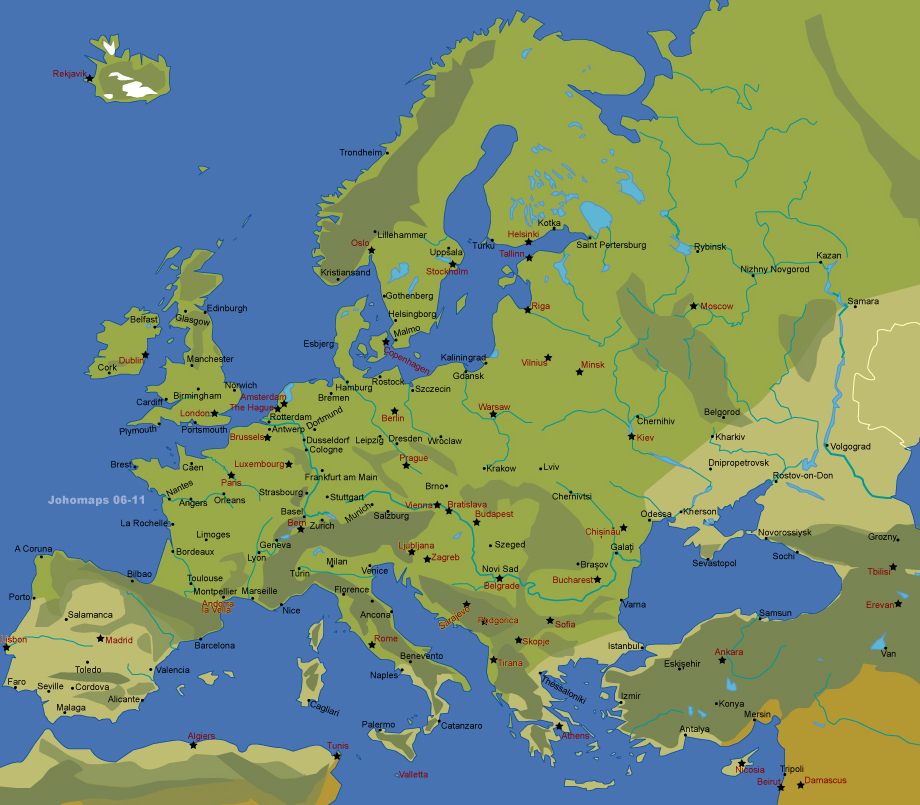
\includegraphics[scale=0.4]{europecities}

%Capítulos extra
\backmatter
\chapter{Las 20 ciudades europeas más baratas para mochileros (en euros)}

\begin{enumerate}
	\item Sofia, Bulgaria - 18.39
	\item Cracovia, Polonia - 19.72
	\item Belgrado, Serbia - 19.76
	\item Riga, Letonia - 20.26
	\item Kiev, Ucrania - 22.14
	\item Sarajevo, Bosnia y Herzegovina - 22.34
	\item Bucarest, Romania - 23.49
	\item Budapest, Hungría - 24.73
	\item Varsovia, Polonia - 26.18
	\item Bratislava, Eslovaquia - 28
	\item Estambul, Turquia - 31.34
	\item San Petersburgo, Rusia - 31.50
	\item Praga, República Checa - 33.70
	\item Zagreb, Croacia - 33.68
	\item Moscú, Rusia - 35.74
	\item Tenerife, España - 37.90
	\item Tallin, Estonia - 41.84
	\item Lisboa, Portugal - 43.38
	\item Berlín, Alemania - 46.80
	\item Atenas, Grecia - 47.50
\end{enumerate}
\end{document}